%%%%%%%%%%%%%%%%%%%%%%%%%%%%%%%%%%%%%%START PREAMBLE THAT IS THE SAME FOR ALL EXAMPLES
\documentclass{article}

%Required: You must have these
\usepackage{Sweave}
\usepackage{graphicx}
\usepackage{tabularx}
\usepackage{hyperref}
\usepackage{natbib}
\usepackage{pdflscape}
\usepackage{array}
\usepackage{gensymb}
%\usepackage[backend=bibtex]{biblatex}
%Strongly recommended
  %put your figures in one place
%\SweaveOpts{prefix.string=figures/, eps=FALSE} 
%you'll want these for pretty captioning
\usepackage[small]{caption}

\setkeys{Gin}{width=0.8\textwidth}  %make the figs 50 perc textwidth
\setlength{\captionmargin}{30pt}
\setlength{\abovecaptionskip}{10pt}
\setlength{\belowcaptionskip}{10pt}
% manual for caption  http://www.dd.chalmers.se/latex/Docs/PDF/caption.pdf
%Optional: I like to muck with my margins and spacing in ways that LaTeX frowns on
%Here's how to do that
 \topmargin -1.5cm        
 \oddsidemargin -0.04cm   
 \evensidemargin -0.04cm  % same as oddsidemargin but for left-hand pages
 \textwidth 16.59cm
 \textheight 21.94cm 
 %\pagestyle{empty}       % Uncomment if don't want page numbers
 \parskip 7.2pt           % sets spacing between paragraphs
 %\renewcommand{\baselinestretch}{1.5} 	% Uncomment for 1.5 spacing between lines
\parindent 0pt% sets leading space for paragraphs
\usepackage{setspace}
%\doublespacing

%Optional: I like fancy headers
%\usepackage{fancyhdr}
%\pagestyle{fancy}
%\fancyhead[LO]{How do climate change experiments actually change climate}
%\fancyhead[RO]{2016}
 
%%%%%%%%%%%%%%%%%%%%%%%%%%%%%%%%%%%%%%END PREAMBLE THAT IS THE SAME FOR ALL EXAMPLES

%Start of the document
\begin{document}

%\SweaveOpts{concordance=TRUE}
 \bibliographystyle{..//..//refs/bibstyles/amnat.bst}
\title{Supplemental materials for Spatial and temporal shifts in photoperiod with climate change} % perspective paper for OSPREE analyses

\author{A.K. Ettinger, D. Buonaiuto, C. J. Chamberlain, I. Morales-Castilla, E. Wolkovich}
%\date{\today}
\maketitle  %put the fancy title on
%\tableofcontents      %add a table of contents
%\clearpage

%goal is GCB Opinon

%%%%%%%%%%%%%%%%%%%%%%%%%%%%%%%%%%%%%%%%%%%%%%%%%%%
\renewcommand{\thetable}{S\arabic{table}}
\renewcommand{\thefigure}{S\arabic{figure}}

\section*{Supplemental Methods}

\par \textbf{The Observed Spring Phenology Responses in Experimental Environments (OSPREE) database}
\par The OSPREE database is a compilation of 72 controlled environment studies of budburst responses to temperature and photoperiod, and spans 39 years and 203 woody plant species \citep{wolkovich2019}.  To identify studies for the database, we searched ISI Web of Science and Google Scholar with the following terms: 
\begin{enumerate}
\item TOPIC = (budburst OR leaf-out) AND (photoperiod or daylength) AND temperature*, which yielded 85 publications

\item TOPIC = (budburst OR leaf-out) AND dorman*, which yielded 193 publications

The initial searches yielded 201 papers, which were reviewed. OSPREE includes the subset of those studies that focus on temperate woody plants, tested for photoperiod and/or temperature effects on budburst, leafout, or flowering, and for which we could quantitatively identify forcing, photoperiod, and chilling treatments.

\end{enumerate}\par \textbf{Quantifying and mapping differences in green-up across the United States and Europe (Figure 2)}
\par Satellite images can be combined with algorithms---e.g. MODIS Land Cover Dynamics---to identify the dates on which phenophases transition from one to the next. Using data from the MODIS sensor (available at:  https://lpdaacsvc.cr.usgs.gov/appeears/), we extracted spatial data for North American and Western European green-up---the beginning of seasonal greening---for the years 2009 and 2012. Green-up dates are calculated on the basis of the onset of the Enhanced Vegetation Index \citep{huete2002}. From green-up maps for each year, we derived the photoperiod corresponding to each pixel (according to its geographic coordinates and day of the year), using the R function ``daylength" in package geosphere (see Figure 2a,b in main text). Finally, we mapped spatial patterns of temporal shifts in green-up by comparing an early and late spring years. To do so, we subtracted the 2013 green-up map from the 2009 one (Figure 2c). Thus, a negative difference signifies earlier green-up in 2012 versus 2009;  a positive difference is the result of later green-up in 2012 compared with 2009. The spatial resolution corresponding to the maps is 0.1 x 0.1 degrees.
%% IMC - I'm not sure what level of detail we want to give here. Let me know if you want me to be more explicit/clear.



\par \textbf{Mapping temporal and spatial shifts in space and time (Figure 3)}
\par To examine the range of photoperiod treatments imposed in growth chamber experiments of woody plants, and compare these treatments to shifts in photoperiod that may be expected due to climate change-induced spatial and temporal shifts, we identified all experiments in the OSPREE database with at least two photoperiod treatments; this resulted in 30 experiments \citep[Table \ref{tab:eff},][]{wolkovich2019}. 
\par We wanted to compare experimental photoperiod treatment levels in these 30 experiments to temporal shifts that would be required for species to experience equivalent photoperiod shifts with climate change. To do this, we identified the dates between the winter and summer solstices on which daylengths at the latitude of the experiments matched treatment levels. When no date matched the experimental treatment level exactly, we chose the date with the most similar daylength, as long as it was within 0.5 hours of the photoperiod treatment level. For studies with only two photoperiod treatment levels, we identified matching dates for both levels. For studies with more than two daylength treatments, we identified matching dates for the lowest treatment level and the second lowest treatment level (e.g., if treatment levels were 10, 12, 14, and 16 hours of daylight, we identified dates with 10 and 12 hours of daylength only). This provided an estimate for the minimum temporal shift required during the spring that would equal the difference between the two treatments; that is, the minimum difference, in days, between dates with the lower daylength treatment and dates with higher daylength treatment.
In 11 out of 30 cases, the difference between in experimental treatments exceeded what the range in photoperiod experienced across the entire year at the study latitude (Xs in Figure 3). Note that many studies occur at high latitudes, which experience a wide range of photoperiod across the year. 

\par To compare differences between experimental photoperiod treatment levels to differences in photoperiod species would experience with spatial shifts, we identified the daylength on the summer solstice for the latitudes of all 30 experiments in Table \ref{tab:eff}. To get potential changes in daylength experienced, we compared the summer solstice daylength at each latitude to the daylength on latitudes up to 40 degrees poleward (in continuous increments of 0.1\degree). Because latitudinal variation in daylength is greatest during the solstices, this provides a maximum possible shift in daylength, at a constant day of year. We then matched the experimental change in photoperiod between two treatments levels to the latitudinal shift that provided an equivalent change in photoperiod. In 13 out of 30 cases, the experimental treatment differences exceeded the photoperiod change that would be experienced with a latitudinal shift of up to 40\degree (Figure 3). 

\par The experiments assessed may not have originally aimed at assessing effects of climate change on phenological responses, yet in many cases, treatments do occur at scales that could be relevant for understanding spatial and temporal shifts in photoperiod with climate change (Figure 3). It is striking, however, that there are also many studies with treatments that are well-outside the expected or possible range of change (Figure 3).  To be most relevant for understanding implications of photoperiod shifts with climate change, future studies should consider the range of potential photoperiod shifts that are likely to occur in nature as experimental treatment levels are designed.

\par \textbf{Nonlinearities in phenological responses to daylength (Figure 4)}
\par To explore the extent to which spring phenology responds linearly (or non-linearly) to photoperiod, we selected OSPREE publications that had three or more photoperiod treatments, and, after reading the methods of these papers in detail, identified three that used three or more photoperiod treatments in the same experiment: \citet{Ashby:1962aa}, \citet{Heide:1993a}, and \citet{Caffarra:2011b}. \citet{Ashby:1962aa} used two North American populations of \textit{Tilia america}. \citet{Heide:1993a} studied populations of \textit{Fagus sylvatica} from Basel, Switzerland; Copenhagen, Denmark; As, Norway; and the Carpathian Mountains, Poland. \citet{Caffarra:2011b} used plant material of \textit{Betula pubescens} from Wexford, Ireland. These experiments all used forcing temperatures of 21 or 22\degree C. Chilling varied considerably across experiments, and chilling level was categorized as follows:
\begin{itemize}
\item <1 Chill Portions = None
\item 1-44 Chill Portions = Low
\item 45-69 Chill Portions = Medium 
\item 70-106 Chill Portions = High
\item >106 Chill Portions = Very High
\end{itemize}

\par Emerging patterns suggest that non-linear responses that differ across species and that may interact with varying chilling (Figure 4). It is important to recognize, however, that the sample of studies reviewed is limited taxonomically, occurs across a narrow range of forcing temperatures, and spans only three papers. A better understanding of photoperiod responses requires additional experimental work conducted across a range of photoperiod treatments, ideally spanning diverse taxa.

\par \textbf{Comparing shifts in experienced photoperiod in experiments to those in the natural world with climate change (Figure 5)}
\par We took current budburst estimates (1981-2000) from PhenoFit \citep{duputie2015} and projected budburst (2081-2100) using the A1Fi Phenofit scenario for two species -- \textit{Fagus sylvatica} and \textit{Quercus robur} -- and compared these points to data obtained from OSPREE. The OSPREE data points were collected from experiments and days of budburst were calculated from the start of the experiment, rather than from the start of the year. In order to render these points comparable to the PhenoFit current estimates and projections, we re-scaled the OSPREE days to budburst by adding the day of budburst from the first Phenofit observation to all of the OSPREE data points. We only used PhenoFit estimates that had both current and projected estimates. Note that the three OSPREE data points for \textit{Quercus robur} with extremely high days to budburst (right panel of Figure 5 in the main text) were from an experiment with very low forcing temperatures \citep[][3.8-5.7$^{\circ}$]{Morin:2010aa}. 

\bibliography{/Users/aileneettinger/Documents/GitHub/ospree/refs/ospreebibplus}
\clearpage
\section* {Supplemental Tables}
\begin{footnotesize} 
% latex table generated in R 3.6.0 by xtable 1.8-4 package
% Wed Jun  3 21:41:27 2020
\begin{table}[ht]
\centering
\caption{\textbf{Locations, photoperiod treatments, and whether or not photoperiod had an effect on budburst}, in studies in the OSPREE database with at least two photoperiod treatments. These studies span 176 different woody species and are mapped in Figure 3. In the `photoperiod effect' column, `yes' denotes studies in which authors report significant photoperiod effects on at least one focal species; `no' which denotes nonsignificant effects of photoperiod.} 
\label{tab:eff}
\begingroup\footnotesize
\begin{tabular}{|p{0.22\textwidth}|p{0.07\textwidth}|p{0.12\textwidth}|p{0.07\textwidth}|p{0.07\textwidth}|p{0.15\textwidth}|p{0.1\textwidth}|}
  \hline
reference & study & continent & latitude (\degree) & longitude (\degree) & daylength range (hrs) &  photoperiod effect? \\ 
  \hline
\citet{Ashby:1962aa} & exp1 & North America & 42.99 & -89.41 & 8-16 & yes \\ 
  \citet{Basler:2014aa} & exp1 & Europe & 46.31 & 8.27 & 9.2-16 & yes \\ 
  \citet{Caffarra:2011b} & exp2 & Europe & 52.32 & -6.93 & 10-16 & yes \\ 
  \citet{Falusi:1990aa} & exp1 & Europe & 46.03 & 10.75 & 9-13 & no \\ 
  \citet{Falusi:1996aa} & exp3 & Europe & 38.27 & 15.99 & 9-13 & yes \\ 
  \citet{Ghelardini:2010aa} & exp1 & Europe & 43.72 & 11.37 & 8-16 & no \\ 
  \citet{Heide:2005aa} & exp1 & Europe & 56.18 & -4.32 & 10-24 & yes \\ 
  \citet{Heide:2008aa} & exp1 & Europe & 48.40 & 11.72 & 10-24 & yes \\ 
  \citet{Heide:2011aa} & exp1 & Europe & 59.67 & 10.67 & 10-20 & no \\ 
  \citet{Heide:2012aa} & exp1 & Europe & 56.50 & -3.06 & 10-24 & yes \\ 
  \citet{Heide:2015aa} & exp2 & Europe & 56.50 & -3.06 & 10-15 & yes \\ 
  \citet{Heide:1993a} & exp1 & Europe & 59.50 & 10.77 & 8-24 & yes \\ 
  \citet{Heide:1993a} & exp1 & Europe & 59.67 & 10.83 & 8-24 & yes \\ 
  \citet{Heide:1993a} & exp3 & Europe & 47.50 & 7.60 & 13-16 & yes \\ 
  \citet{Howe:1995aa} & exp1 & North America & 40.55 & -124.10 & 9-24 & yes \\ 
  \citet{Laube:2014a} & exp1 & Europe & 48.40 & 11.71 & 8-16 & no \\ 
  \citet{Myking:1995} & exp1 & Europe & 56.10 & 9.15 & 8-24 & yes \\ 
  \citet{Nienstaedt:1966aa} & exp1 & North America & 44.17 & -103.92 & 8-20 & yes \\ 
  \citet{Okie:2011aa} & exp1 & North America & 32.12 & -83.12 & 0-12 & yes \\ 
  \citet{Partanen:2001aa} & exp1 & Europe & 61.93 & 26.68 & 6-16 & yes \\ 
  \citet{Partanen:2005aa} & exp1 & Europe & 61.82 & 29.32 & 5-20 & yes \\ 
  \citet{Partanen:1998aa} & exp1 & Europe & 60.03 & 23.05 & 8.66-12 & yes \\ 
  \citet{Pettersen:1972aa} & exp1 & Europe & 59.66 & 10.77 & 10-24 & no \\ 
  \citet{Sanz-Perez:2009aa} & exp1 & Europe & 40.40 & -3.48 & 10-16 & yes \\ 
  \citet{Vihera-Aarnio:2006aa} & exp1 & Europe & 60.45 & 24.93 & 16-17 & yes \\ 
  \citet{Vihera-Aarnio:2006aa} & exp1 & Europe & 67.73 & 24.93 & 20-21 & yes \\ 
  \citet{Vihera-Aarnio:2006aa} & exp2 & Europe & 60.45 & 24.93 & 15-19 & yes \\ 
  \citet{Vihera-Aarnio:2006aa} & exp2 & Europe & 67.73 & 24.93 & 22-23 & yes \\ 
  \citet{Worrall:1967aa} & exp3 & North America & 41.31 & -72.93 & 8-16 & yes \\ 
  \citet{zohner2016} & exp1 & Europe & 48.16 & 11.50 & 8-16 & yes \\ 
   \hline
\end{tabular}
\endgroup
\end{table}\end{footnotesize} 
\clearpage
\section* {Supplemental Figures}

\begin{figure}[h]
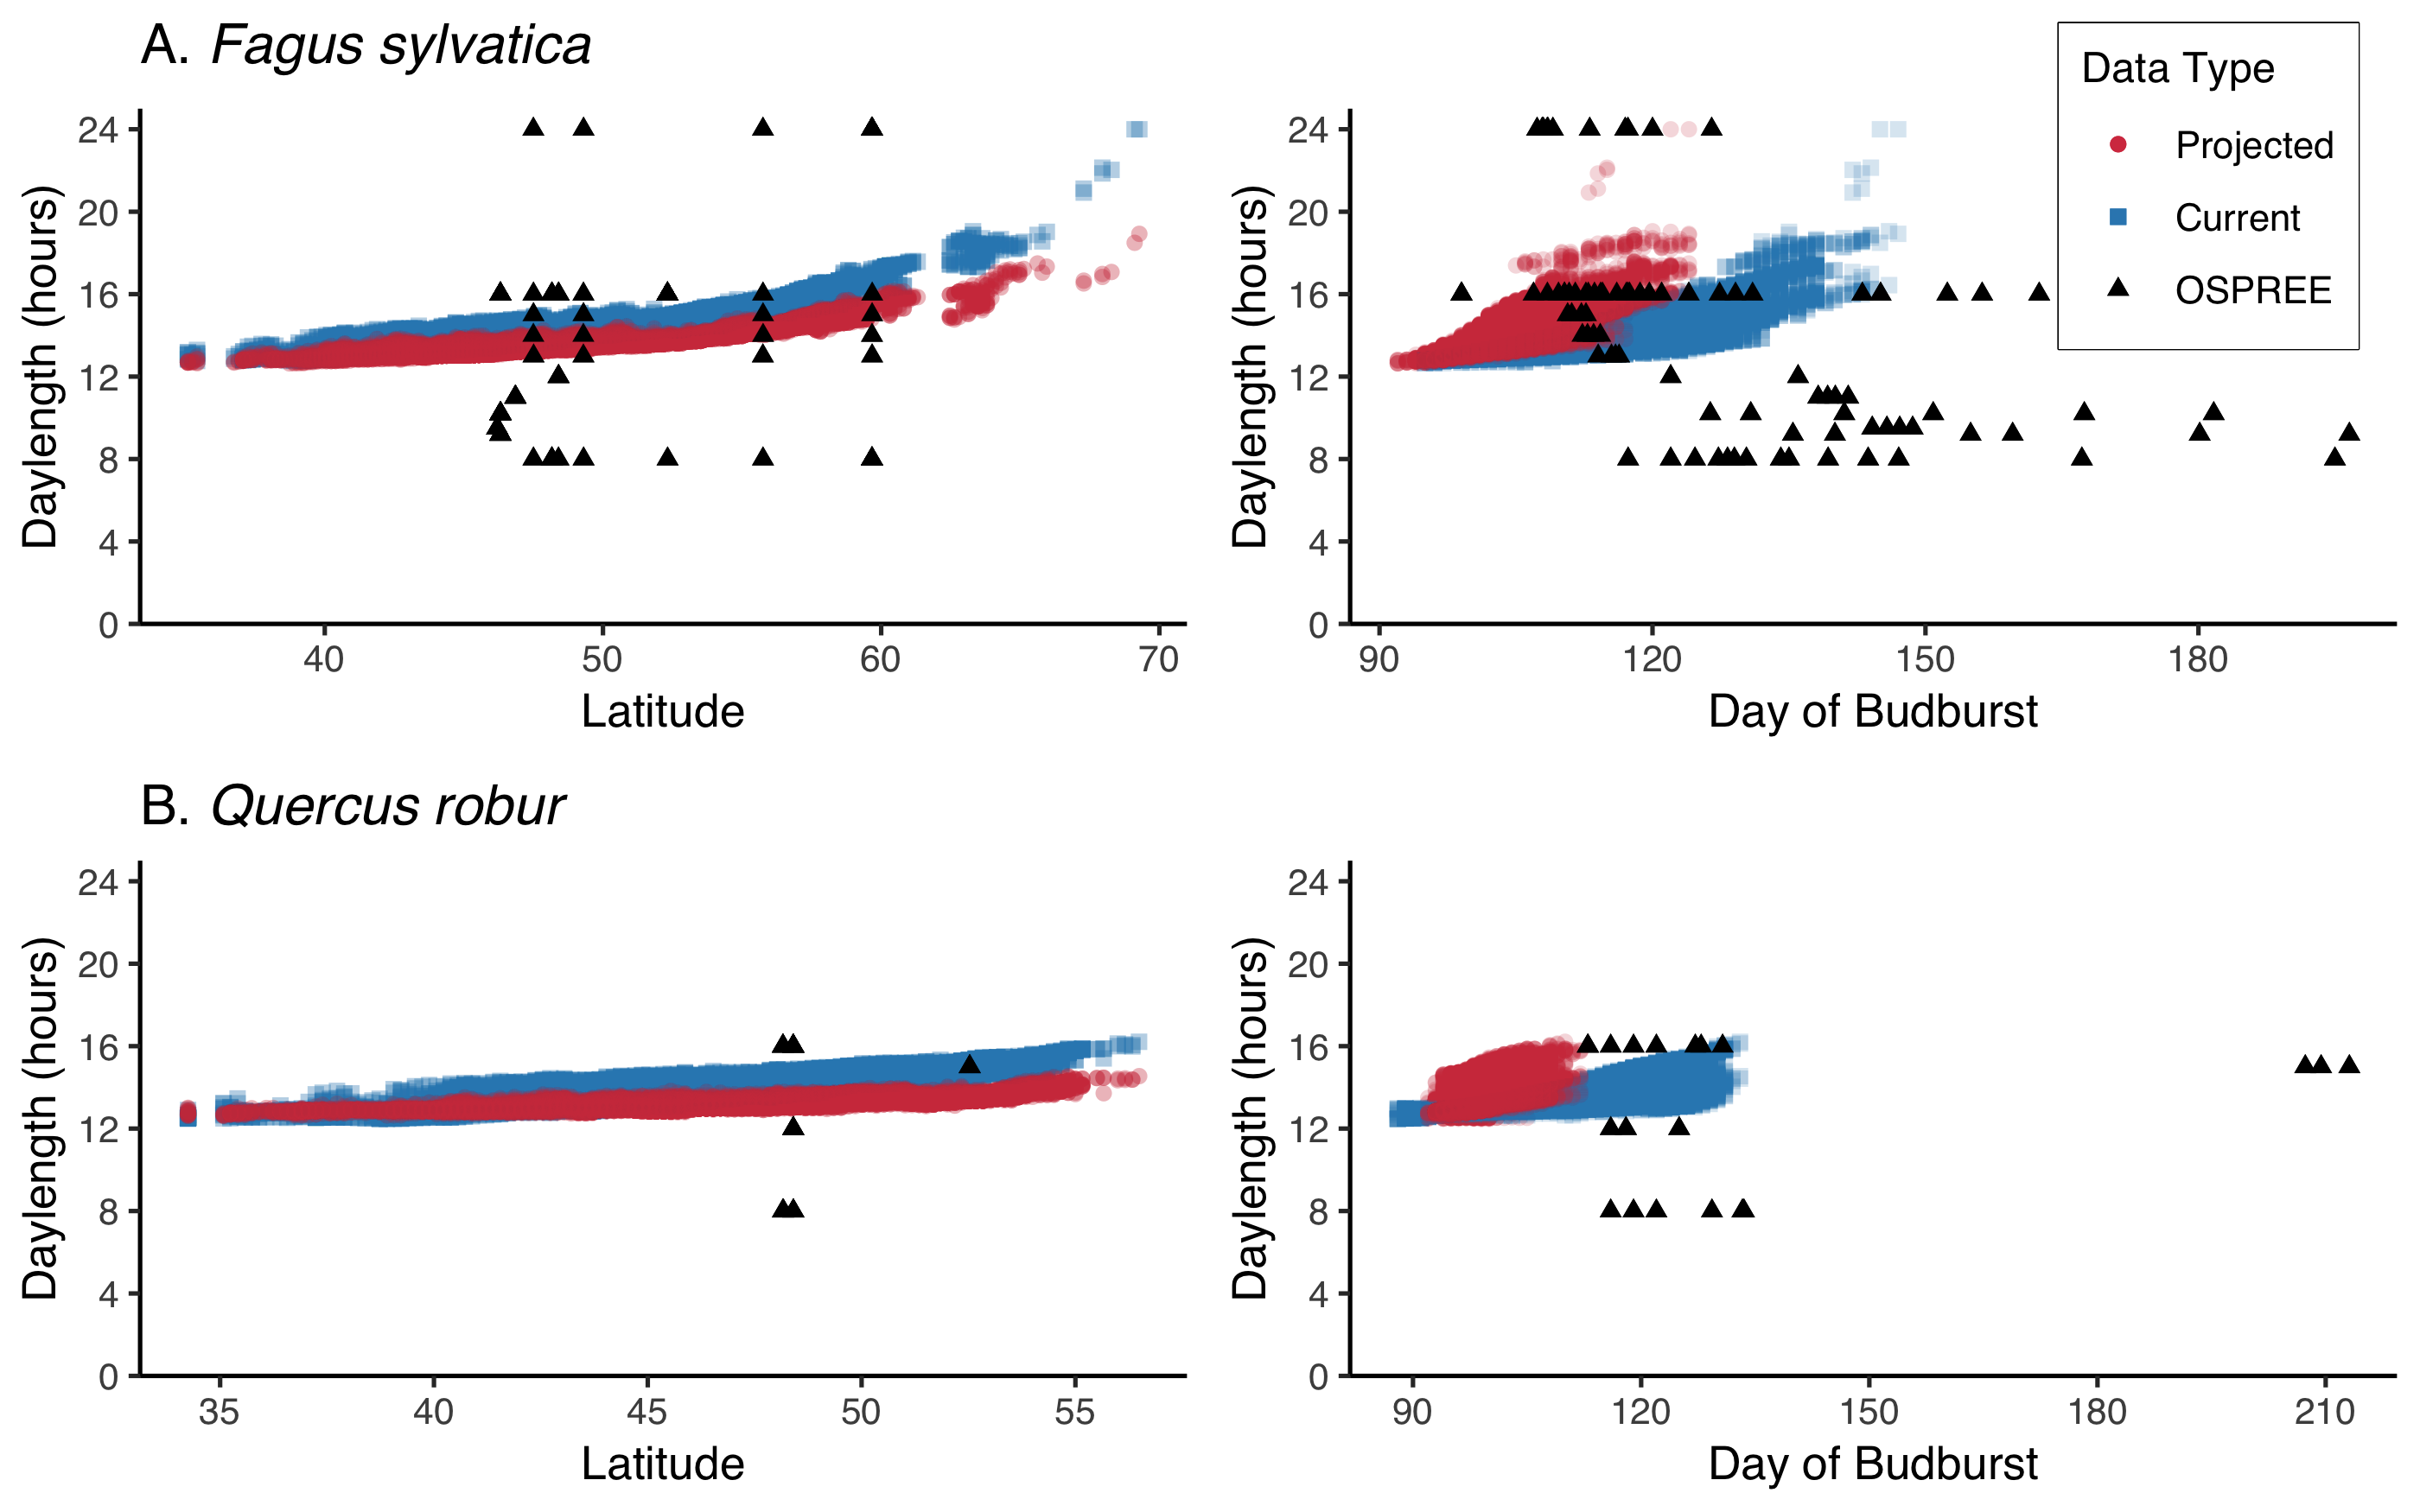
\includegraphics{..//..//analyses/photoperiod/figures/2D_actual_combined.png} 
\caption{\textbf{Experienced photoperiods in growth chamber experiments differ from those in the natural world}, shown here by latitude (left panels) and by day of budburst (right panels) for \emph{Fagus sylvatica} (A, upper panels) and \emph{Quercus robur} (B, lower panels). Triangles show experimental treatments of photoperiod in the OSPREE database (Box 1). To illuminate potential gaps between experiments and the natural world, we show the photoperiod when budburst occurs in its current (1981-2000) and projected ranges \citep[2081-2100, using the A1Fi Phenofit scenario, see][]{duputie2015}. We scaled the days to budburst for all OSPREE data points by adding the day of budburst from the first Phenofit observation. See Supplemental Materials and \citet{duputie2015} for additional details.} 
 \label{fig:fagus}
 \end{figure}
 
 
%%%%%%%%%%%%%%%%%%%%%%%%%%%%%%%%%%%%%%%%
\end{document}
%%%%%%%%%%%%%%%%%%%%%%%%%%%%%%%%%%%%%%%%
